\documentclass[12pt]{article}
\usepackage{graphicx}
\openup 1em

\title{Munchies Incorporated}
\date{2017-03--5}
\author{Lucas Arias\
        \and
        Chuck Coleman\
        \and
        Nora Cook\
        \and
        TJ Mitchell
        }
\begin{document}
        \maketitle
        \newpage
\section{Purpose}
        \indent Munchies Inc. is a business dedicated to making review sites for 
        small businesses. We will also be developing services for file storage and
        email that small businesses can take advantage of. These services will 
        allow small business to be more efficient without the need for a costly 
        in-house solution.\\

        The main focus of Munchies Inc. is our website Welp. This website 
        will act as a service for Alfred residents to find information about local 
        businesses. It will include menus and prices for restaurants and will 
        also allow reviews for registered users. The website will help locals 
        become more aware of local businesses and boost their business. It will 
        also empower the consumer by giving them more information products they
        may want to buy.\\

        Along with a public website, we will also offer file storage 
        allowing businesses to save money by using less paper. It will also help 
        organization as there will be no papers to lose.\\

        We will also have email services available. Having a private email 
        service will help businesses keep information secure and more private 
        rather than using a public service such as gmail.\\

\section{Shareholders}
        Shareholders will be able to buy the file sharing and email services by
        emailing or calling us and getting a quote. These services will be private
        and will not be publicly available. The website Welp will be completely
        public and open for anyone to use, barring any users that may be banned
        due to harrasment or hate speech in the reviews. 

\section{Milestones}
        \subsection{Overview}
                This section will go over the technical aspects of the 
                project,  detailing what we need to develop and eventually the 
                release date of the various technologies. This will cover all 
                servers being used and all software that will be developed. The 
                website Welp will be developed by Nora Cook and Chuck Coleman while
                Lucas Arias and TJ Mitchell will handle the servers and networks. 

        \subsection{Welp}
                Welp will be developed independently while the servers are
                being set up. It will be a full stack application made with the 
                following technologies: PHP for the front end, Apache webserver, 
                and MySQL database and database server. The application will also
                be source controlled using git and hosted with github. 

        \subsection{Active Directory}
                %TODO, find out info from TJ and Lulu
                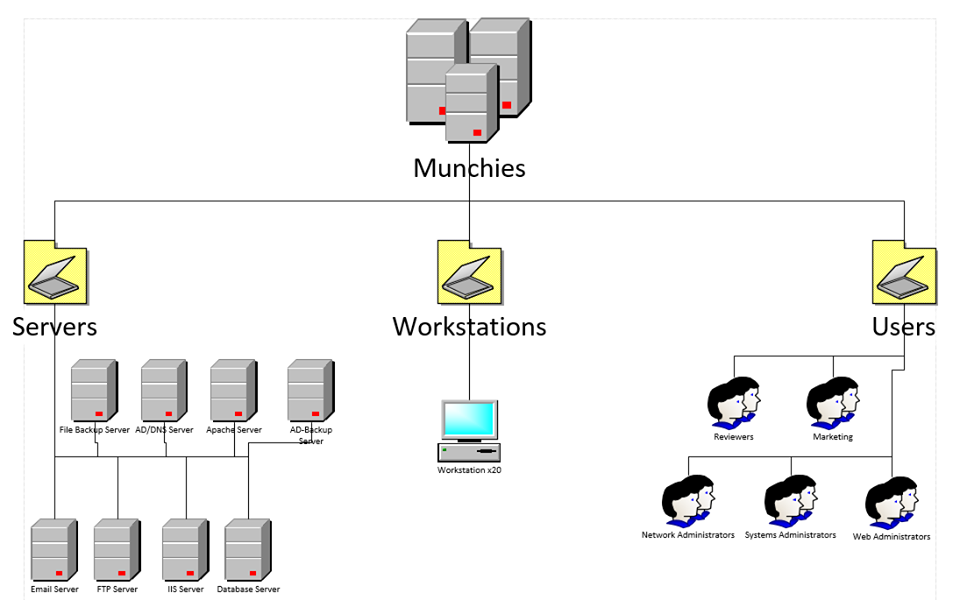
\includegraphics[width=15cm, height=12cm]{activedirectory.png}

        \subsection{Networks}
                %TODO, find out info from TJ and Lulu
                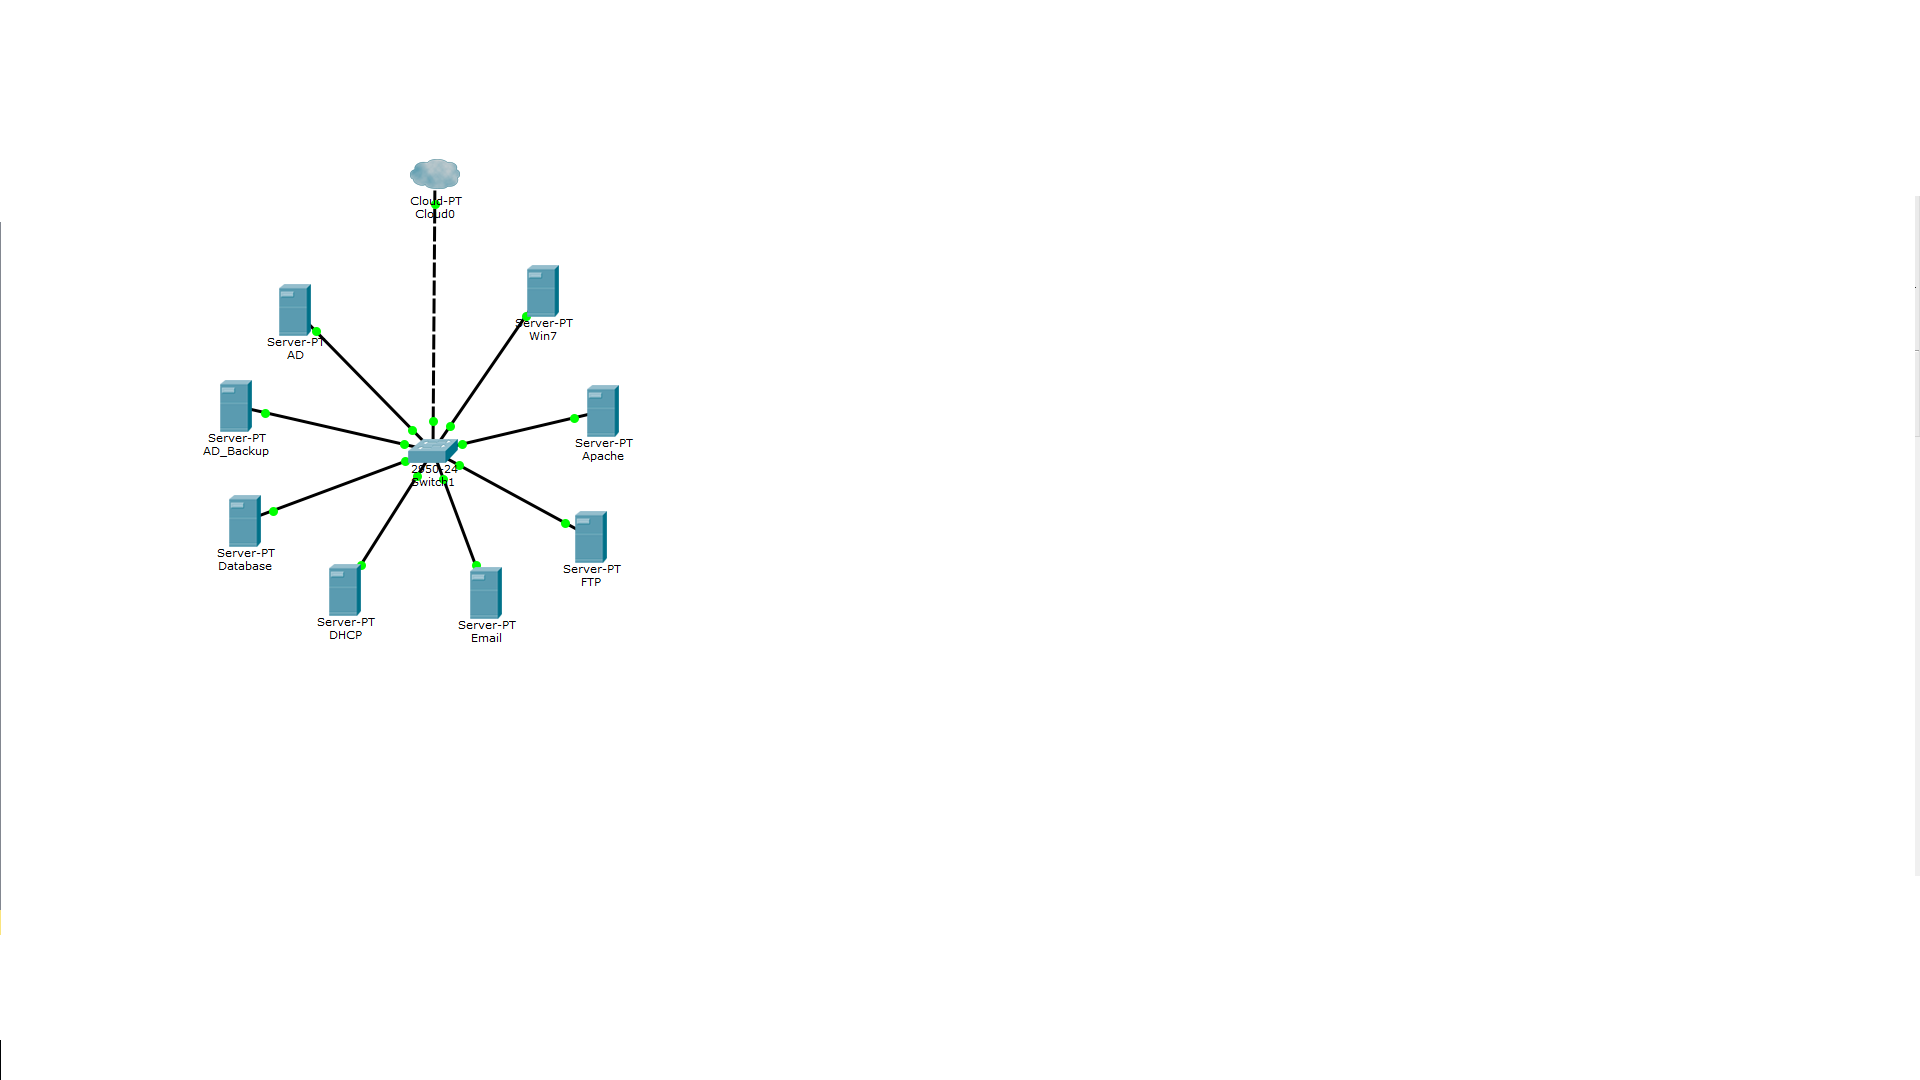
\includegraphics[width=15cm, height=12cm]{topology.png}

\newpage
\section{Glossary}
        \subsection{PHP}
                PHP is a hypertext preprocessor used to quickly create websites
                dynamically. This will be the language of choice for development.

        \subsection{Apache}
                Apache is a web server that can be run on both Linux and Windows.
                It is extremely powerful and offers features for security and will
                allow for the website to be accessed from any web browser.

        \subsection{MySQL}
                MySQL is a database that is free and open source and also includes
                a server. This will allow us to put our database on a seperate 
                server, making it more secure.

        \subsection{Full Stack}
                Full stack means that the application includes everything from
                the database to the front end.

\end{document}
